\documentclass[11pt]{article}
\usepackage{lscape, longtable, underscore, graphics, graphicx}
\usepackage{geometry, amsmath} 
\usepackage[table]{xcolor}
\marginparwidth = 0pt

\begin{document}
\begin{flushleft}
Puget Sound Regional Council\\
\today
\end{flushleft}

\vspace{1cm}
\begin{center}
{\Large \bf Fitting Spline Curves to LUV Ranges} 
\end{center}
%
\section{Data and Objectives}
%
For each of the 148 jurisdictions, there are time series data on population and employment that include two observed data points, namely 2010, 2013, and two future estimates, namely 2040 (further called {\em second time estimate}) and one of 2025, 2030, 2031 or 2035 (further called {\em first time  estimate}). Both future estimates are given as ranges, i.e. in form of a lower and upper bound.

The goal is to fit a spline such that it intersects exactly the observed data and is contained within the lower and upper bound of the future estimates. We define two criteria for the curves:
\begin{enumerate}
\item minimizing the curvature
\item maximizing the slope
\end{enumerate}
For example, in the following figure, the red curve is preferable to the black curve, as it has less curvature and a higher slope.
\begin{center}
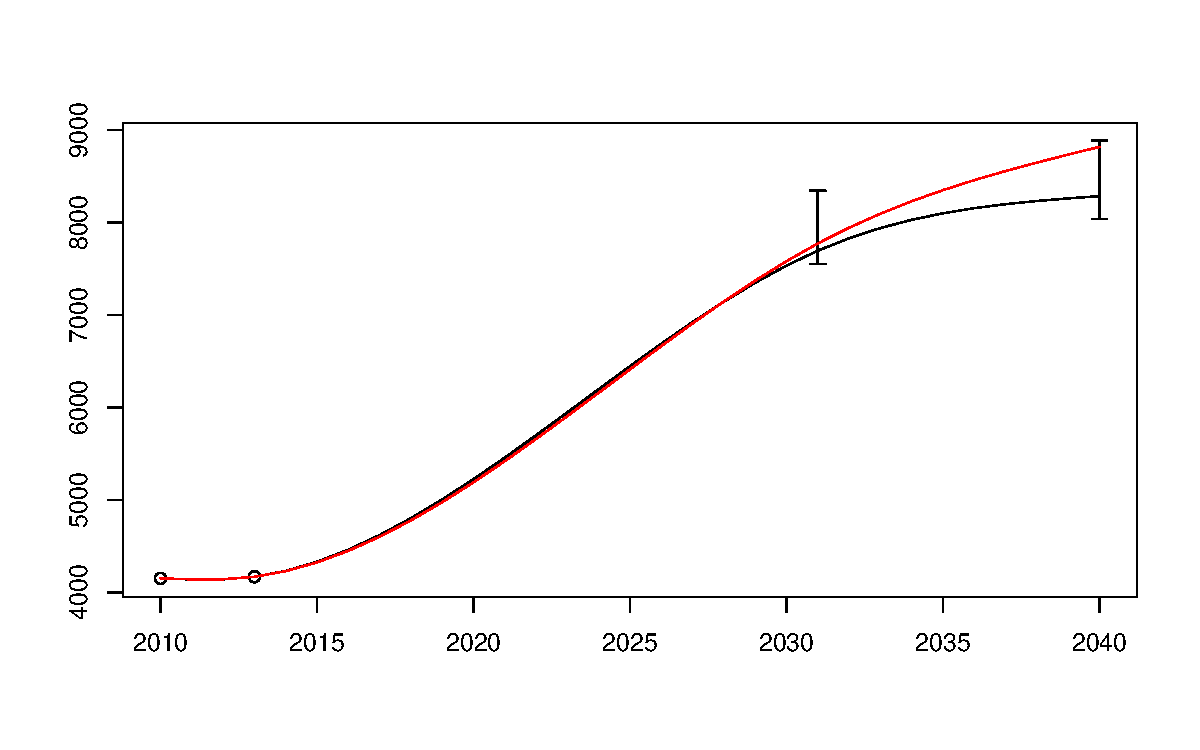
\includegraphics[scale=0.5]{methexamplecurves.pdf}
\end{center}

\pagebreak
%
\section{Methodology}
%
A simple methodology is used in which we create a large amount of possible splines and choose the one that fits our criteria best. Curvature is measured using the second derivative of the curve; for the slope the first derivative is used. 

More specifically, the procedure consists of the following steps:
\begin{enumerate}
\item Randomly select $n$ points between the lower and upper bound of the first time estimate, say $a_1, \dots, a_n$.
\item Randomly select $n$ points between the lower and upper bound of the second time estimate, say $b_1, \dots, b_n$.
\item Randomly select $R$ combinations of pairs $c_l=(a_i, b_j)$, where $R \leq n^2, \, l=1,\dots,R$.
\item Attach each of $c_1,\dots, c_R$ to observed data points and perform a natural spline interpolation for all remaining years. This results in $R$ curves.
\item For each such curve remove data points up to 2013 and obtain the mean of the first derivatives on the remaining time points. Denote it by $d^{(1)}_1, \dots, d^{(1)}_R$.
\item For each curve remove data points up to 2013 and the last point of the curve, i.e. 2040, and obtain the mean of the second derivatives of the remaining time points. Denote it by $d^{(2)}_1, \dots, d^{(2)}_R$.
\item Since we want to maximize $d^{(1)}$ and minimize $d^{(2)}$, we select the curve for which $\max_{1\leq i \leq R} \frac{d^{(1)}_i}{d^{(2)}_i}$.
\end{enumerate}
Setting $n=100$ and $R=1000$ yields reasonable results.


\vspace{1cm}
\begin{flushleft}
For questions on the methodology contact:\\
Hana \v{S}ev\v{c}\'{\i}kov\'{a}\\
hsevcikova@psrc.org
\end{flushleft}

\end{document}  